
Posiadanie wielu obrazów wiąże się z potrzebą ich przeglądania i porównywania.
Należy, więc posiadać jakieś narzędzie do wyświetlenia w sposób poprawny, najlepiej jednym i tym samym programem.

\subsection{Przeglądarki obrazów}

Przeglądarki obrazów to programy należące do kategorii przeglądarki plików.
Zwykłe przeglądarki obrazów takich jak jpg, png lub gif wyświetlają obraz w takiej postaci jakiej jest zapisany, oczywiście najpierw przeprowadzają dekompresje obrazu.
W przypadku obrazów medycznych najczęściej nie mamy do czynienia z danymi reprezentującymi kolory w spektrum światła widzialnego.
Przeglądarka obrazów DICOM musi wygenerować kolorowy obraz z danych na podstawie parametrów obrazu.

\subsection{Porównanie przeglądarek obrazów}

Trudno jest porównywać coś tak złożonego jak przeglądarka obrazów medycznych, nie można jednoznacznie powiedzieć, że jedna jest lepsza od drugiej. W celu porównań wyróżniono 26 kryteriów do porównywania przeglądarek w postaci „tak” lub „nie”, podzielonych na 5 grup, platformy, interfejsu, wsparcie, obrazowanie dwu i trój wymiarowego.
Kryteria te w jasny sposób pozwalają na ocenę praktycznych aspektów użytkowania przeglądarki.

\paragraph{Platforma}

Samodzielność, aplikacje samodzielne są zaprojektowane tak, aby nie wymagały żadnego dodatkowego sprzętu fizycznego bądź infrastruktury do poprawnego działania(np. systemu Windows oraz serwisów przez niego dostarczanych).
Rozwiązania sieciowe, określają czy aplikacja jest usługą sieciową i można z przeglądarki korzystać jak ze strony WWW.
Wieloplatformowość, możliwość uruchomienia ich na różnych systemach operacyjnych Linux/MacOS/Windows
Rozwiązania mobilne, możliwość używania na urządzeniach mobilnych takich jak telefon.

\paragraph{Interfejs}

Przeglądarka powinna mieć możliwość komunikacji z interfejsami innych systemów.
Podstawowe interfejsy sieciowe to: C-STORE SCP DICOM C-STORE, C-STORE SCU, Query-Retrieve, WADO, Parameter Transfer.

\paragraph{Wsparcie techniczne}

Dokumentacja, dostępność pisemnej dokumentacji oprogramowania (np. podręczniki lub strony internetowej).
Wsparcie przez pocztę internetową, możliwość porozumienia się z twórcą lub opiekunem oprogramowania.
Forum, możliwość pytania się społeczności o opinie i ich wymiana.
Wiki, strona internetowa w formacie Wikipedii dostępna dla użytkownika.

\paragraph{Obrazowanie dwu-wymiarowe}

Przewijanie(\fromEng{scroll}), proces wyświetlania obrazów, można poprawić dzięki zmniejszeniu interakcji z klawiaturą oraz myszką. Można to osiągnąć na przykład, oferując możliwość przejścia do następnego lub poprzedniego obrazu przez przesunięcie kółkiem myszy lub używając przycisków góra/dół na klawiaturze.
Metadane, przeglądania powinna obejmować analizowanie i wyświetlanie metadanych obiektów DICOM, powinna obejmować wyświetlanie rozdzielczości obrazu, badanie (np. identyfikator podmiotu) oraz znaczniki DICOM specyficzne dla dostawcy (np. specjalne ustawienie urządzenia rejestrującego).
Warstwa informacyjna, najważniejsze informacje powinny powinny być wizualizowane w oknie wyświetlacza jako nakładka na obraz.
Na przykład aktualna pozycja lub nazwa podmiotu wykonującego badanie.
Okienkowanie (okna cyfrowe), sposób zamiany danych na skale szarości, okienkowanie jest opisane w sekcji \ref{sec:windowing}.
Pseudo-kolorowanie obrazu, tabele (LUT, \fromEng{LookUpTable}) odwzorowujące szare wartości obrazu na pseudo-kolory, poprawiaja one czytelność obrazu.
Histogram, histogramy wizualizują wystąpienia i rozkład wartości kolorów na obrazach, pozwalają opisywać istotne cechy obrazu
Wymiarowanie, możliwości rysowania bądź zaznaczania linii lub innych kształtów do analizy i wyznaczania odległości w jednostkach długości na obrazie.
Jest to możliwe gdyż nagłówki pliku DICOM zawierają parametry sprzętowe urządzenia (np. ilość pikseli na centymetr).
Adnotacje(opisy), które były wytworzone przez personel medyczny powinny być zapisywane w odpowiedni sposób w pliku.

\paragraph{Obrazowanie trój-wymiarowe}

Rekonstrukcja wtórna, zwykle dane dotyczące objętości medycznej są gromadzone wzdłuż jednej osi ciała (np. poprzecznej).
W wielu przypadkach ważne jest przeglądanie danych w innych kierunkach (np. strzałkowych lub czołowych), aby poprawić wizualizację niektórych struktur.
W tym celu należy zapewnić funkcjonalność rekonstrukcji osi pomocniczej na podstawie kierunku pierwotnego.
Plastry objętości kostki(\fromEng{Slice Cube Volume}), przekroje mogą być lepiej wyświetlane w określonej pozycji.
Funkcjonalność kostki plasterka umożliwia niezależną regulację położenia różnych osi wycinków (np. poprzecznych, strzałkowych lub czołowych) w modelu objętościowym.
Podczas tego przekroje są pokazane w osobnym oknie.
Renderowanie objętościowe – dane obrazu 3D są bezpośrednio wizualizowane jako objętość.
Użytkownik może wchodzić w interakcje z woluminem poprzez obracanie lub skalowanie.
Transfer Function(nie znam polskiej nazwy), służy do odwzorowania wartości szarości obrazów wokseli na wartości krycia typów tkanek (np. kości). Struktury obrazu pasujące do wzorców szarych wartości są podświetlone. Niewykorzystane szare wartości są wyświetlane jako
przezroczyste. Specyficzne struktury stają się lepiej widoczne.
Generowanie powierzchni, dzięki różnym algorytmom można generować powierzchnie w postaci wokselów. Reprezentacje powierzchni można również zastosować do poprawy wizualizacji niektórych struktur obrazu.

\subsection{Funkcje przeglądarki obrazów}

\subsubsection{Obsługa wielu formatów danych}

Standard DICOM przewidział możliwość zapisania danych w różnych formatach.

\subsubsection{Podstawowe operacje na obrazie}

\begin{itemize}
      \item Skalowaniu lub powiększenie.
            Możliwość powiększenia lub zmniejszenia wyświetlanego obrazu o pewny współczynnik skalujący.

      \item Przesuwanie(\fromEng{pan})
            Możliwość przesuwania obrazu o dowolny wektor.
            Przydatne gdy powiększymy obraz do takiego stopnia, że nie będzie mieścił się na ekranie lub w okienku programu.

      \item Lupa, skalowanie miejscowe
            Możliwość miejscowego powiększenia obrazu.
            Przykład użycia takiego narzędzia znajduje się na rysunku \ref{fig:wyswietlanie001}.

            \begin{figure}[!htbp]
                  \caption{Przykład narzędzia Lupa w przeglądarce \href{https://www.softneta.com/products/meddream-dicom-viewer/}{MedDream DICOM Viewer}.}
                  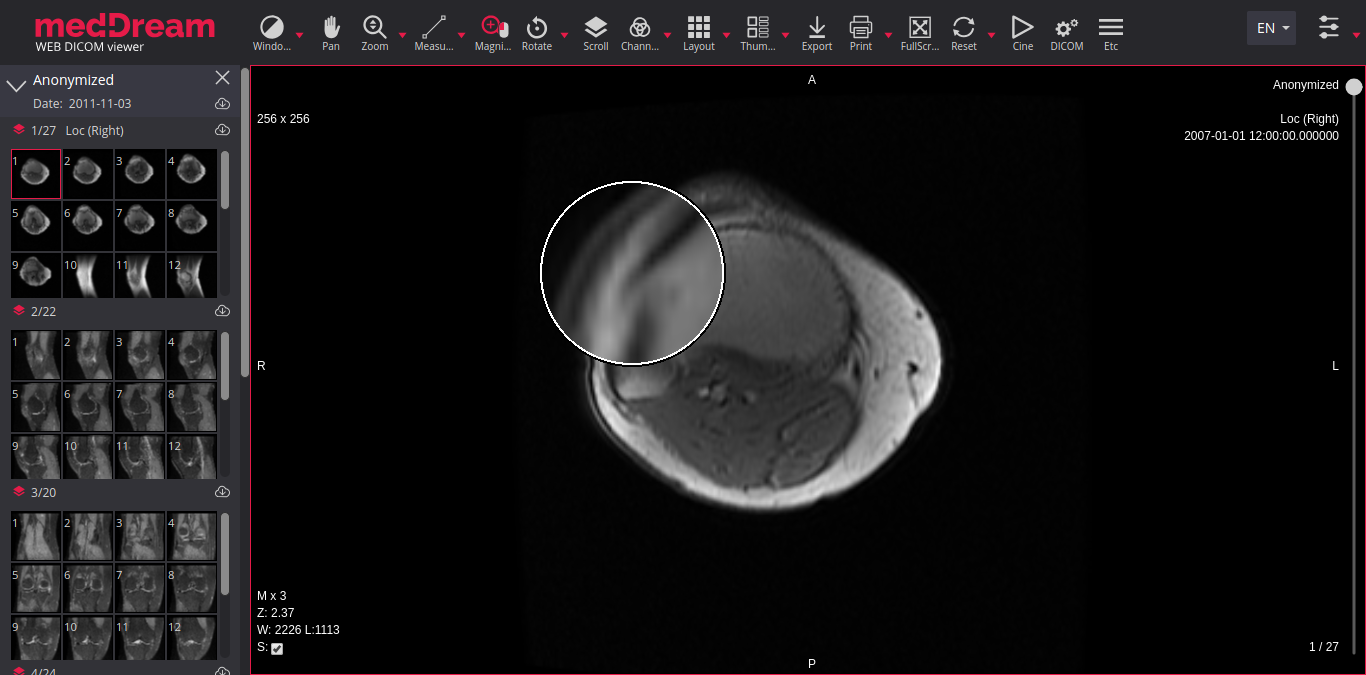
\includegraphics[width=\textwidth]{img/wyswietlanie001.png}
                  \centering
                  \label{fig:wyswietlanie001}
            \end{figure}

      \item Rotacja i odbicia lustrzane
            Możliwość obrócenia obrazu o zadany kąt.
            Oraz możliwość odbicia lustrzanego obrazu w dwóch osiach X i Y.

\end{itemize}

\subsubsection{Analiza parametrów w celu lepszej informacji}

\begin{itemize}
      \item Okienkowanie.
            Termin odnosi się do używania funkcji okna cyfrowego w celu zamiany obrazu danych na obraz monochromatyczny możliwy do wyświetlenia.
            Okienkowanie jest szczegółowo opisane w sekcji \ref{sec:windowing}.

      \item Maski lub nakładki(\fromEng{overlay}).
            Możliwość nałożenia maski, elementu, który będzie przysłaniał fragment obrazu w celu lepszej wizualizacji bądź ukrycie mało wartościowych obiektów, np. tła.
\end{itemize}

\subsubsection{Obsługa wielu plików}

\begin{itemize}

      \item Obsługa DICOMDIR.
            Możliwość wczytania pliku DICOMDIR i wyświetlenie struktury serii badań.

      \item Wczytanie wielu plików i ich połączenie w formie filmu.
            Możliwość wczytania wielu plików z tej samej serii, ułożenia ich według pozycji geometrycznej i wyświetlenia ich jako film.
            Czyli periodyczna podmiana obrazu na obraz następny w serii.

      \item Wyświetlanie wielu obrazów jednocześnie.
            Możliwość wyświetlenia obrazów w postaci kratki, w której każda komórka była by innym obrazem.

            Przykład wyświetlenia wielu obrazów na raz w jednym oknie znajduje się na rysunku \ref{fig:dicomviewer001}

            \begin{figure}[!htbp]
                  \caption{Przykład wyświetlenia wielu obrazów na raz w jednym oknie w przeglądarce \href{https://www.santesoft.com/win/sante-dicom-viewer-3d-pro/sante-dicom-viewer-3d-pro.html}{Sante DICOM Viewer 3D Pro}}
                  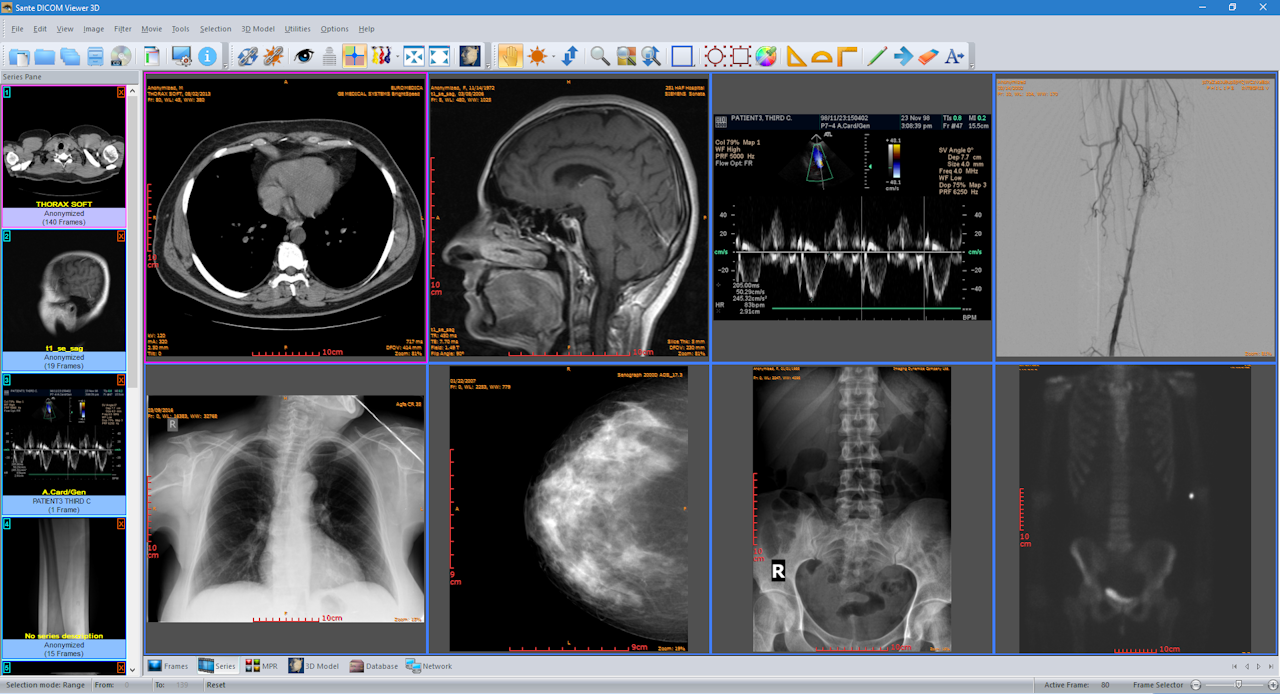
\includegraphics[width=\textwidth]{img/dicom-viewer-001.png}
                  \centering
                  \label{fig:dicomviewer001}
            \end{figure}
\end{itemize}

\subsubsection{Generowanie obrazów woliumetrcznych}

Jeżeli mamy do dyspozycji wiele obrazów tomograficznych o znanych parametrach to możemy wczytać je, posegregować a następnie wygenerować trój-wymiarowy obiekt a następnie wyświetlić go na ekranie komputera za pomocą trójwymiarowej grafiki komputerowej.

Przykład takiego obrazu znajduje się na rysunku \ref{fig:dicomviewer002}.

\begin{figure}[!htbp]
      \caption{Przykład generowania obrazów 3D z wielu obrazów tomograficznych w przeglądarce \href{https://www.santesoft.com/win/sante-dicom-viewer-3d-pro/sante-dicom-viewer-3d-pro.html}{Sante DICOM Viewer 3D Pro}}
      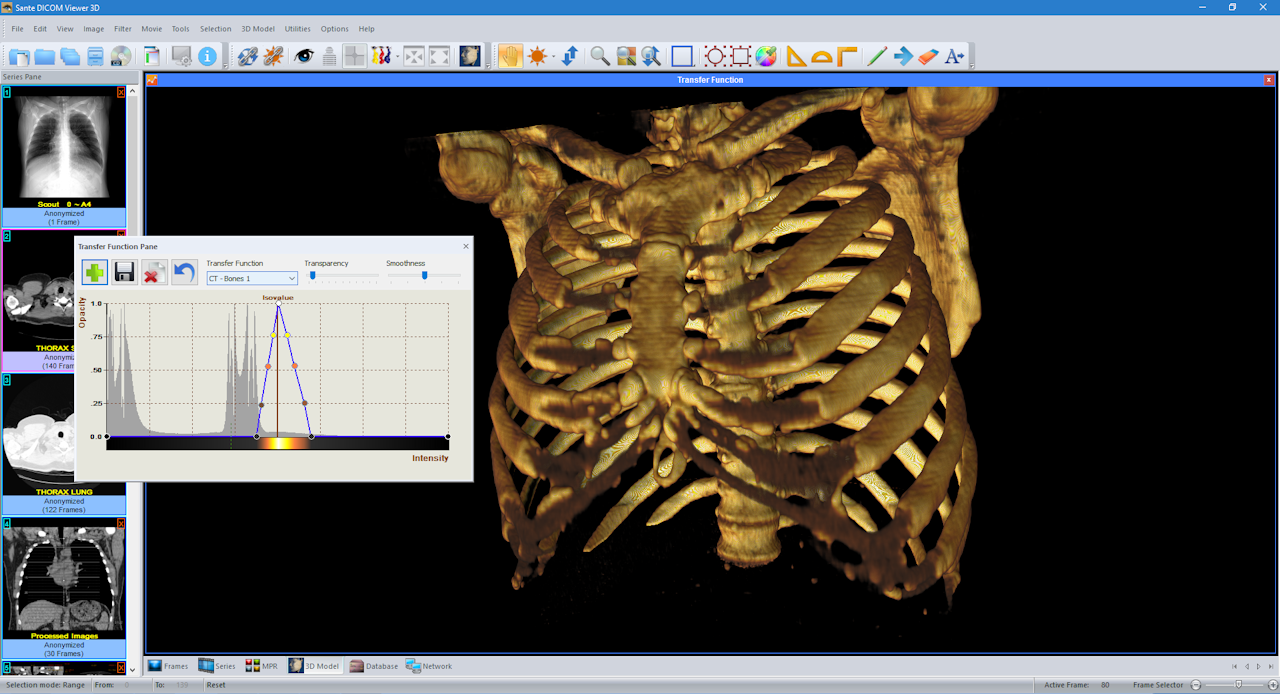
\includegraphics[width=\textwidth]{img/dicom-viewer-002.png}
      \centering
      \label{fig:dicomviewer002}
\end{figure}

\subsubsection{Analiza i przetwarznie danych}

\begin{itemize}
      \item Histogram
            Możliwość wygenerowania histogramu obrazu.

            Histogram to wykres przedstawiający dystrybucje wartości numerycznych obrazu.

      \item Mierzenie obrazu, wykonywanie pomiarów
            Możliwość zmierzenia odległości pomiędzy dwoma punktami przez lekarza lub zmierzenia wielkości/pola zadanego kształtu.

      \item Tworzenie obrazów transwersalnych.
            Obrazy tomograficzne obrazują przekroje, jeżeli parametry wielkości woksela są dostępne to istnieje możliwość wygenerowania nowego obrazu który byłby obrazem ułożonym w poprzek.

            Przykład generowania obrazów transwersalnych jest pokazany na rysunku \ref{fig:dicomviewer003}

            \begin{figure}[!htbp]
                  \caption{Przykład generowania obrazów transwersalnych w przeglądarce \href{https://athenadicomviewer.com/}{Athena DICOM Viewer}}
                  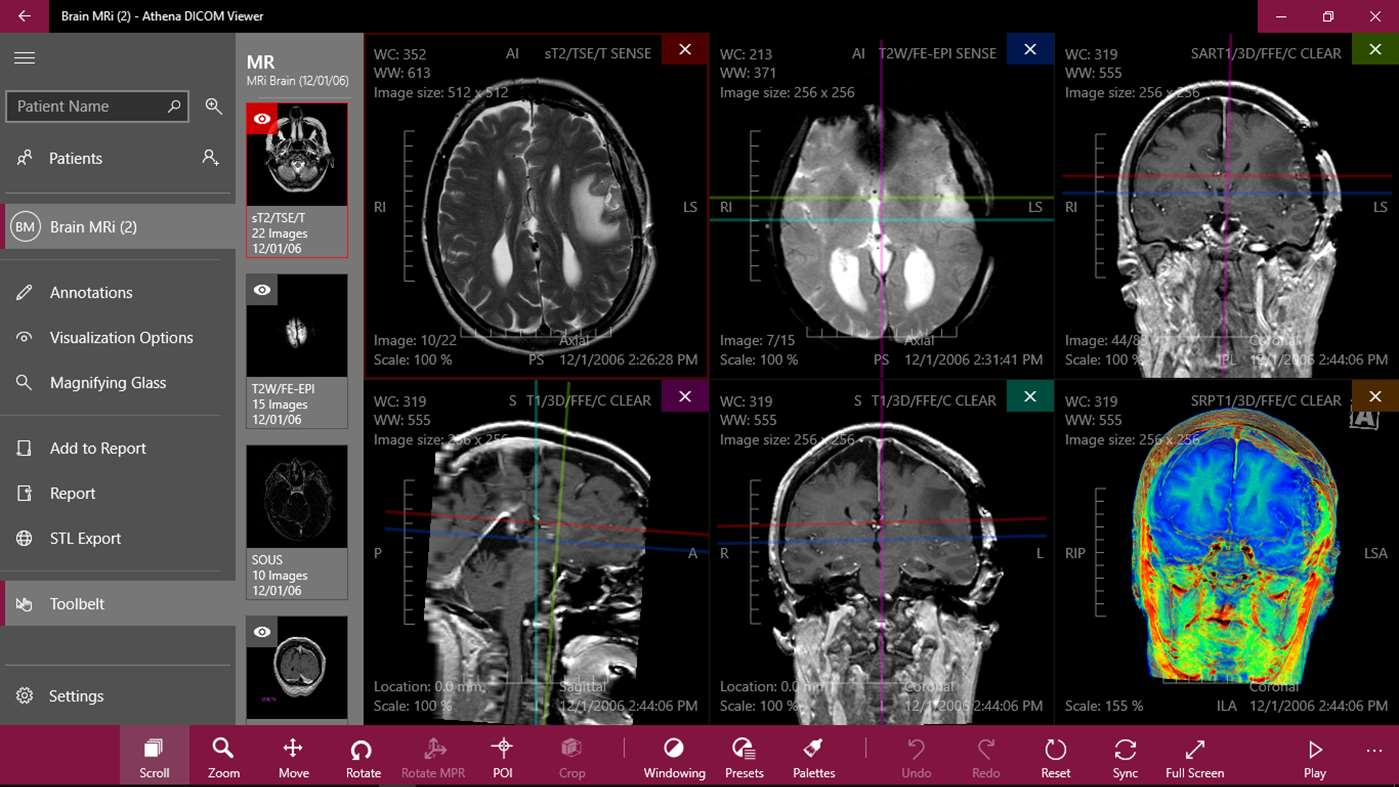
\includegraphics[width=\textwidth]{img/dicom-viewer-003.jpeg}
                  \centering
                  \label{fig:dicomviewer003}
            \end{figure}
\end{itemize}

\subsubsection{Edycja danych}

\begin{itemize}
      \item Dodawanie nowych obiektów.
            Możliwość rysowania, dodawania figur geometrycznych lub tekstu przez lekarza i możliwość zapisu tych informacji w pliku DICOM.
            Chodzi tu głównie o szkice i notatki tworzone podczas analizy obrazu przez personel medyczny.

      \item Edycja Parametrów oraz anonimizacja danych.
            Możliwość edycji parametrów w poliku DICOM w różnych celach.
            Najczęściej funkcja jest używana do usuwania danych osobowych pacjenta w celu poźniejszej publikacji obrazu.

\end{itemize}

\subsection{Możliwości mojej przeglądarki}

Po analizie możliwości przeglądarek plików DICOM dostępnych na rynku postanowiłem zaimplementować następujące komponenty w mojej przeglądarce:

\begin{itemize}
      \item Przesuwanie(\fromEng{pan})

      \item Skalowaniu lub powiększenie

      \item Rotacja i odbicia lustrzane

      \item Okienkowanie

      \item Obsługa wielu formatów zapisu

            \begin{itemize}
                  \item Monochrome
                  \item RGB
                  \item YBR
            \end{itemize}

      \item Wczytanie wielu plików i ich połączenie w formie filmu
\end{itemize}

Moją przeglądarkę nazwałem Sokar.